\documentclass{article}
\usepackage[utf8]{inputenc}
\usepackage{amsmath}
\usepackage{geometry}
 \geometry{
 a4paper,
 total={160mm,240mm},
 left=25mm,
 top=25mm,
 }
\usepackage{graphicx}
\usepackage{caption}
\usepackage[parfill]{parskip}
\usepackage [english]{babel}
\usepackage [autostyle, english = american]{csquotes}
\MakeOuterQuote{"}
\usepackage{abstract}
\renewcommand{\abstractnamefont}{\normalfont\Large\bfseries}
\usepackage{titling,lipsum}
\usepackage{url}
\title{Internal Facing Performance Analysis Report}
\begin{document}
\begin{titlingpage}
\maketitle
\vspace{1cm}
{\scshape\Large An evaluation of the PolarDrive control system Performance \par}
\hrulefill \par 
\vspace{15cm}
{\scshape \textbf{Les Schaffer PhD} \,\,-\,\,  \par}
{\scshape \textbf{Luke Rickert MSc} \,\,-\,\, \par}
\end{titlingpage}
\tableofcontents
\newpage
\section*{Introduction}
This report undertakes an multifaceted evaluation of PolarWork's internally developed motion control technology and will include a detailed description of the constituent components in the PolarWorks portfolio, a description of relevant motion control technology, and a comparison of the PolarWorks motion strategy with existent competing systems via simulations and other measures. The results of this undertaking will be used to identify motion control applications where PolarWorks technologies may be best applied to help guide future research and development and how the PolarWorks approach should be positioned in the market from a technical grounding. 
\section{Generalized Control System Performance Criteria}
In order to accurately and impartially evaluate the performance of the various motion control systems it is necessary to establish criteria using easily measured data which characterize each system's relative performance. For completeness evaluation should also consider such factors as cost, energy efficiency and suitability to particular applications (for example low speed, high load vs high speed, low load). The initial comparison will use the same motor with differing control and motor drive methodologies to simplify the comparison.  

\subsection{Measurable Physical Performance}
Working definition is RMS (Root Mean Square) deviation from desired value. This "value" may be position, velocity, acceleration etc. 
\subsection{Other Considerations}
It general terms it is unlikely that a fully developed and properly designed brushless servo system (AC or DC) will ever provide inferior performance to any stepper based motion control system, be it open or closed loop. This performance advantage comes at a considerably higher price in terms of motors, control, drives and encoders therefore for certain low cost applications traditional steppers may be more appropriate. For example simply sourcing a high resolution encoder for a servo will cost more than an entire nema 17 stepper drive and motor. Among the servos implementations there will be differences in performance based on the control algorithms, this is likely to be the most valuable portion of the evaluation for non-low cost applications. 
\par
Although initial investigations will utilize the same motor with differing control approaches future (more refined) considerations will compare differing types of motors, encoders etc along with a range of control methodologies, therefore each systems considered should be optimized. For example an AC servo with gear reduction and a brake might be compared to a stepper motor with neither. Obviously the comparison must also include the difference in cost, complexity etc otherwise the most expensive and most complicated option will in all likelihood be shown to be universally superior. These other factors include system consider cost as mentioned but also complexity, reliability, easy of implementation (manual vs automatic tuning etc), customization, application flexibility. Additionally the performance evaluation should include aspects such as path efficiency, computing power requirements, convergence rate, maximum overshoot (standard deviations perhaps), steady-state error and control robustness (the ability to recovery and accuracy under peak loads and perturbations). 
\section{Existing Technology}
Over the last 50 or so years, many advanced motion control theories and approaches have been presented in academia yet due to limits in the then available technology such as computing power, sensor technology and other factors including limited market demand and general industry conservatism most of those proposed approaches remain under exploited today. The complete technology package under development by PolarWorks which will take in computer generated part data, and then create machine instructions based on those data and the physics of the machine to simulate, optimize, and control offers the opportunity to bring modern high performance manufacturing and motion control technology quickly and easily into the real world.  The PolarWorks approach can use technology developed internally as well as exiting and future approaches as called for by the requirements of the particular application. The core value presented by PolarWorks is in the creation of a unified system that can use the best available technology, it is not necessarily any one component of the system.  

\subsection{Motion Control Theory}
The field of motion control is mature and diverse. There are a wide range of existing approaches, some of which are quite similar to those proposed by PolarWorks. The range of control approaches is following in the following list. 
\par
List of the main control techniques (adapted from Wikipedia \footnote{September 2018 \url{https://en.wikipedia.org/wiki/Control_theory} } )
\begin{itemize}
\item Adaptive control 
\item A hierarchical control 
\item Intelligent control (artificial neural networks, Bayesian probability, fuzzy logic, machine learning) 
\item Optimal control such as Model Predictive Control (MPC) and linear-quadratic-Gaussian control (LQG) 
\item Robust control which explicitly handles uncertainty 
\item Stochastic control
\item Energy-shaping control 
\item Self-organized criticality control 
\end{itemize}
\par
A detailed examination of these approaches is beyond the scope of this document but an awareness of the existing approaches is help in situating the PolarWorks approaches into widely understood language and also to identify how any novel developments which the PolarWorks provides over the existing available technology. 
\par 
It appears that the most appropriate categorization for PolarDrive is as an MPC subset of Optimal Control. MPC can be defined by the following \footnote{September 2018 \url{https://en.wikipedia.org/wiki/Model_predictive_control}} 
\begin{quote}
Model Predictive Control (MPC) is a multi-variable control algorithm that uses:
\begin{itemize}
\item An internal dynamic model of the process
\item A history of past control moves and
\item An optimization cost function over the receding prediction horizon to calculate the optimum control moves.
\end{itemize}
\end{quote}
\par
There is value in understanding the range of motion control methodologies and techniques available as it allows the possibility of both situating the internally developed control systesms within the existing technology and also helps to match the correct control approach with each particular application.
\par
\subsection{Motion Control System Simulation}
Motion control simulation is an existing technology although there are no known existing options which are directly and fully equivalent to the proposed scope of TestBench. There are however commercial and open source simulation programs which are similar in execution. Such programs include JModelica which use the Modelica modeling language \footnote{\url{https://www.modelica.org/}} for modeling, simulating, optimizing and analyzing complex dynamic systems. This is worth noting as this language may provide a an open and more or less standard means of characterizing electomechanical components in a similar way as SPICE parts are used for electronic circuit design and simulation. This could be Incorporated into TestBench both to ease adoption and to reduce the effort required to develop that portion of the software. 
\subsection{Machine Control Language} \label{machinecontrol}
A standardized system of commands is required to communicate the desired path or movements to a machine tool or other electromechanical system under motion control. Currently in industrial applications this system, although not quite standardized, called G-code (ISO 6983). Its history dates back over half a century\footnote{Late 1950's and early 1960's}, and although it generally is functional it is not able to take advantage of the advances in CAD, computing power, sensor and other technology developments since it was created. 
\par 
One proposed new option is STEP-NC \footnote{\url{https://en.wikipedia.org/wiki/STEP-NC}}. Although similar in principle it offers a vastly more information rich machine control language. It also is designed to not only transmit movement commands but also to receive sensor and encoder inputs to allow in-process optimization. With G-code the tool path data, at least in manufacturing applications, is produced by Computer Aided Manufacturing (CAM) software which extracts the tool path from a point cloud which is extracted from 2D drawing or 3D model, this CAM output must be further post-processed for the particular machine and machine controller. This is undesirable as it both separates the tool path from the tool model and any attached information and also because the motion commands that is generates are generally limited to straight line movements and semicircular arcs. A machine control language such as STEP-NC should be capable of providing a more detailed instructions with attached data and use spline based path generation. This new approach may utilize ISO 10303 STEP files as CAD data rather than the point clouds consumed by current CAM software. 
\par 
The advantages of such an approach are non-trivial. For one embedding model information such as Geometric Dimensioning and Tolerancing (GD\&T) requirements provide the option of relieving the CNC operator or CAM engineer from interpreting separate drawings with GD\&T requirements and then manually ensuring that the resulting parts reflect the design intent. Additionally maintaining model integrity through the entire manufacturing process makes quality control much more straight forward and offers the opportunity to integrate checks during the production sequence to monitor machine path deviations etc. Additionally it is at least theoretically possible to avoid the requirement of a customized post processor for each machine and machine controller as is required with G-code. 
\par 
Some more of the advantages of Step-NC were listed in a recent article.\footnote{Journal of Mechanical Science and Technology 32 (7) (2018) 3317~3328}
\begin{quote}
The basic advantages of the STEP-NC in relation to the ISO 6983 (G-code) are the following ones 
\begin{enumerate}
\item A high level of information which is based on the tasks of processing manufacturing features 
\item bi-directional data flow between design and manufacturing without losses
\item object-oriented programming
\item the possibility of processing on some modern CNC machines without the use of post-processors, which are will be eliminated because the interface does not require machine-specific information
\item machine tools are safer and more adaptable
because STEP-NC is independent from the machine tool vendor
\item STEP-NC files can be used for information transfer and enable Web based manufacturing or e-manufacturing
\end{enumerate}
\end{quote}
\par
From the standpoint of compatibility and legacy support TestBench and the other portions of the control system must still be able to work with conventional G-code. It is possible that when combined with full machine simulations the G-code could be analyzed, processed and adjusted for better compatibility with a current machine tool and machine controller requiring no other changes to the process flow. 

\section{PolarDrive System Overview}
In order that it may be evaluated and compared the PolarDrive system must first be described and its functions summarized in some detail. 
\par
The PolarDrive system consists of the following components: 
\begin{itemize}
\item TestBench System Simulation and correlation program
\item Tracer
\item Planner
\item Motor Drive 
\end{itemize}
\par
These components represent the equivalent of the current market process flow of CAM, Post Processor, Machine Controller, and motor drives. It is possible to incorporate some of these these legacy building blocks into the PolarDrive flow if desirable in certain applications.  

\subsection{TestBench Simulation}
TestBench fills the role of the CAM software, machine controller and overall repository of all the control of the software components control components in the system. \par
Along with the control functions it also permits process simulation with full physics and electronic models of a planned system. This can add considerable value to machine development. Properly implemented, simulation has the ability to allow component selection, property adjustment, studies of noise sensitivity, software debugging and other features without the need to first also purchase and build the physical implementations. 
\par 
TestBench is the result of a prototype application used to develop the initial implementation of PolarDrive on a 3D printer. The concept and some components of this software have been used to create a new application which is intended for generalized and flexible application for both internal use and potentially as an external product. This program will not only allow simulation but also will be integrated with the machine control to collect data on the actual performance to allow for simulation correlation, quality control and other potential features. TestBench represents the first part of the PolarDrive integrated chain which will cover all the steps from Model Based Definition (MBD) 3D part data to a finished and QC'ed part.  

\subsection{CAD to CAM Process Flow}
Once the 3D part data has been imported into a motion control system it must be processed to generate machine movements which will create the desired part to the desired tolerances etc. Traditionally this is done in two steps, first the CAD part is imported into a Computer Aided Manufacturing (CAM) program, which then, usually with considerable input from the operator is used to generate G-code tool paths. For the second step these G-code commands are then sent to a post-processor to adjust the G-code for the particular machine and machine controller. Before being actually run on the machine tool this G-code can then be run in a simulator to check for certain errors in the instructions which can result in catastrophic problems in production. 
\par
With the PolarWorks approach there are, potentially at least, multiple means of accomplishing this process of converting a solid CAD part into machine movement. The process flow for the conventional method of consuming G-code from an external CAM program is that the post-processed G-code is read (line by line) into a portion of the control system called the Path Planning Engine (PPE) which translates and processes the commands before sending them to the machine controller called the Tracer which generates spline based paths for the machine tool to follow. 
\par
The primarily alternative offered by and perhaps most valuable portion of a fully vertically integrated motion control system such as PolarWorks is that rather than taking in G-code from an external CAM program it can consume a Model Based Definition (MBD) part directly from a CAD program in a format such as STEP which includes not only the 3D part shape but also tolerances and/or other information.\footnote{Such as Carbon Fiber Reinforced Plastic (CFRP) ply information and orientations for a tape laying machine for aerospace manufacturing.} This MBD part can then be processed internally with full knowledge of the machine tool's drive system and physical and electromechanical characteristics along with the design intent to create seamless tool path for the machine tool. The original MBD can also then be used in the Quality Control (QC) process after part production. This flow is not possible when G-code is imported from CAM software as the G-code instructions are permanently divorced from the original design intent as the path is based on point-cloud conversions of the original part. This new process enables simulation and process optimization to create parts meeting their requirements and avoids or at least minimizes errors caused by flawed post-processors, human error in CAM operations and other potentially costly mistakes.  Step-NC is discussed in more length in section \ref{machinecontrol}. 
\par
There are a range of components in the PolarWorks system that may be combined with TestBench to create a fully integrated CAD-CAM system. (not all portions must be used if there are other options or requirements)

\subsection{Path Planning Engine}
The Pathe Planning Engine (PPE) works in a buffered realm, taking sequential location and velocity data either internal or external CAM software and begins by translating the tool path into the native coordinate system of the machine. Once the points are transformed into the native coordinate system, connecting splines are generated and waypoints are assigned at a predetermined density, along with nominal velocities. The velocities are then optimized by a look-ahead function constrained by an allowable performance envelope, such as maximum acceleration. The waypoint locations and adjusted velocities are then stored in a buffer awaiting a request from the closed loop controller such as the PhysicsModel or Tracer described below. 
\subsection{PhysicsModel}
One means of closed loop feedback control analogous to PID (Proportional–Integral–Derivative) control systems in that it calculates the error from the desired position, velocity, acceleration ... and sends corrected commands to the motor drives. In this case rather than being based on only the error and certain preset coefficients the control system uses a predefined model of the machine, motors, drives and other components to predict the response of the system. Although these sorts of systems, sometimes called Model Predictive Control (MPC) have been long discussed in literature it is only more recently with the proliferation of low cost and high power microcontrollers that this type of control system has become practical for demanding motion control applications. This model of the system would not only be used for real-time control but would be developed and refined in TestBench simulations.

\subsection{Tracer} The Tracer is second conceptual control algorithm used in closed loop motion control. The Tracer's view is limited to the current motion state (as defined by position, velocity, and acceleration) of the tool head and the waypoint it is targeting. The Tracer estimates the time required to reach the waypoint and generates a spline that solves the current motion state to reach the target waypoint. It is worth noting that within PolarDrive it is possible to optimize for many criteria, but currently it is based on minimizing acceleration between points. This optimization is one component of the Iterated Local Jerk Algorithm. The algorithm iterates at specific time intervals between waypoints. For each step, given a target waypoint and current motion state, the algorithm determines a jerk value that will result in the tool traveling along a smooth curve, thereby achieving the waypoint at the specified target velocity. When the current motion state satisfies the waypoint criteria (provided a tolerance value), the algorithm has completed one span (spline between waypoints) and will be provided with a next waypoint from the PPE. 
\subsection{Motor Drive}
PolarDrive is a servo motor drive method developed for stepper and other other motor types. It controls the position of the motor rotor by setting the magnetic field with respect to the rotor using modified sine waves. This approach uses linearized output from the Tracer to compensate for the variations in torque between poles as the motor rotates and other system variations. The result is near silent operation of the motor with linear torque distribution. This and most other servo drive methodologies generally rely on motor or machine axis encoders to provide current motion state information.  
\subsection{PolarDrive definition}
Based on the proceeding description of the motors and control systems PolarDrive may be described as a full feedback type CLSM. When implemented as it is on a hybrid stepper motor, the motors acts a Brushless Synchronous permanent magnet motor driven with a PWM quasi-sinusoidal input. It is important to note that there is nothing about the drive or control approach which limits its application to stepper motors. Future development should explore implementation on other synchronous motors such as BrushLess Direct Current (BLDC) servos and if possible AC servos given their potentially advantageous performance. 

\section{Drive Motors}
There are a range of actuators used in control systems. Most of these are brushless motors such as hybrid steppers and AC servos although other actuators exist such as linear motors although only a range of conventional (rotational) motors will not be considered at the present time. 
\subsection{Conventional Stepper Motor Systems}
A stepper motor is a special type of 2 pole brushless DC (BLDC) motor that is designed with a "toothed" electromagnet so that Pulse Width Modulated (PWM) square wave input will translate into an fixed angular displacements, usually 1.8 or 0.9 degrees. Stepper motors do not have use encoders for feedback and therefore must work by dead-reckoning. A position is reached based on the assumption that a number of steps (or microsteps) will result in a move to the predicted location. Torque is not directly controlled and reduces with velocity which generally limits the speed at which steppers may operate. The trade-off of this that they offer an inexpensive and simple to implement drive system.
\par 
In application most stepper motors are run using microstepping. This allows the motor to turn in smaller increments than the physical steps which generally improves smoothness and accuracy. Although conventionally thought to reduces torque, the actual impact of microstepping on the torque of a motor appears to be non-trivial and is load dependant. Future physical testing will required to better understand this topic beyond what can be gained by simulation. 
\par
In order to avoid or at least minimize performance and accuracy problems associated with missed steps stepper motors must be sized for the peak load which results in relatively larger and more expensive motors than would be needed could they have been sized for more normal operating loads with the ability to correct position via feedback.  Other negative aspects include generally noisy operation, low electrical efficiency and consequent motor heating. Additionally if microstepping is used to increase potential accuracy it reduces the available torque further compounding the limitations for high speed, and or high load applications. Even with microstepping real world accuracy is far more limited than what can be achieved with encoder based feedback systems. Devices which do not have significant operational loads such as low end laser cutters and 3D printers can use stepper motors with the above acknowledged trade-offs. The ability to skip or loose steps can be seen as a safety advantage over a servo that can apply much more than nominal power if a high load (such a crash) is experienced. The importance of this "advantage" is questionable given that there are numerous means to mitigate this danger.  
\par
For relatively small (low power) and moderate accuracy applications stepper motors can offer sufficient performance for a much lower cost than any alternative solution. This is due to a number of factors such as commodity scale of production, simple and interchangeable controllers. The high holding and good low speed torque limit the need for gearing and or brakes further reducing costs. The lack of an encoder is an advantage both in avoiding a potentially expensive part (the encoder) but also in simplifying the control requirements which reduces cost and improves flexibility. (nearly any hybrid stepper may be driven by any driver of the correct sizing with limited tuning, adjustment or software modification. Stepper motors are also usually built on standard (NEMA) mount sizes which aids in interchangeability. With the same mount motors of different lengths (and therefore different torque capabilities) can be easily interchanged. 
\par
It is also possible to drive steppers with feedback using back EMF measurements to improve performance without resorting to physical encoders. Companies such as Trinamic in Germany offer an  example of one such implementation. It is an approach not without compelling advantages over normally driven stepper motors yet still lacks the performance potential of fully implemented, encoder based feedback control systems.  
\par
Stepper motors, along with other brushless motors motors have the advantage over brushed DC motor based servos (by virtue of avoiding brushes which wear, spark and create noise) although this comparison is perhaps invalid given that brushed servos are generally considered obsolete in modern control system design.  
\par 
The following diagram shows a flow chart of the typical stepper motor drive system. 

\begin{figure}[h!]
  \centering
  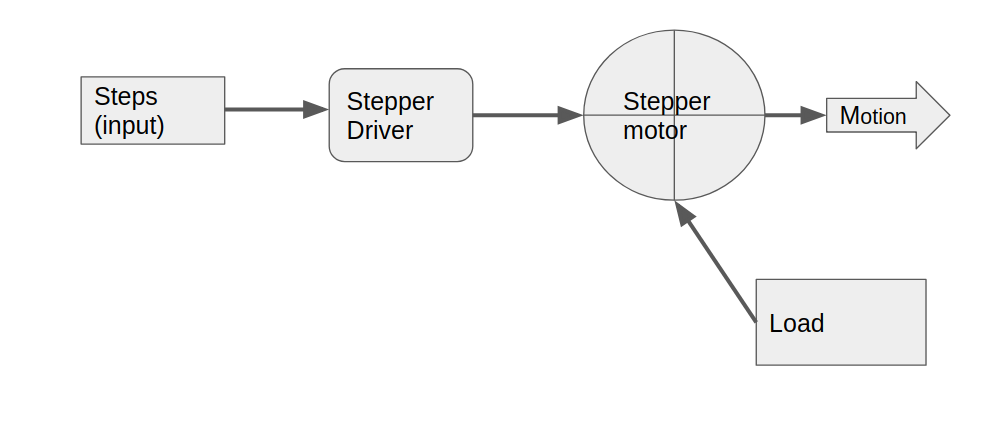
\includegraphics[width=0.8\textwidth]{SM_flow.png}
  \captionsetup{justification=centering}
  \caption{Stepper control Flow}
   \label{fig:SM}
\end{figure}

\subsection{Closed Loop Stepper Motors}
A Closed Loop Stepper Motor (CLSM) is a conventional hybrid stepper motor with encoder added so that it can issue correction moves if it skips or stalls and otherwise improve the control of the motor. Like conventional steppers they have high starting torque, and a relatively low maximum speed and a reduction of torque with rotational velocity.
\par
Closed-loop steppers have higher efficiency and less heating than conventional stepper motors. If an absolute position encoder is used it is removes or minimized the need for the limit switches usually used to define position with conventional stepper motors. Additionally the accuracy is dependent on the encoder resolution rather than the mechanical steps in the motor so if required it can be higher than a conventional stepper motor.
\par 
There is a second class of CLSM, the second type use a more complex feedback system (usually PID) which makes fundamentally makes them servo motors which differentiates them from more basic CLSM implementations which only use the encoder for error correct or end point correction. Being proprietary systems the exact implementation is somewhat difficult to determine and side by side physical testing will be required to fully understand the actual performance and limitations compared to conventional servo motors. The main difference between the second type CLSM will be a reflection of motor architecture, motor drive and feedback mechanism.   
\par
The following shows the control system flow of a servo type CLSM: 

\begin{figure}[h!]
  \centering
  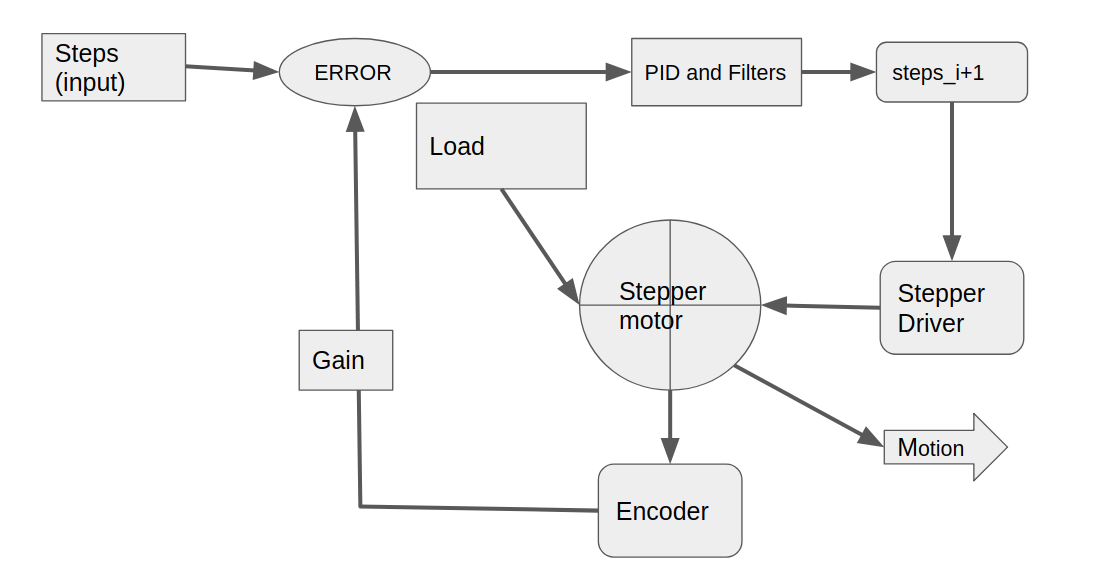
\includegraphics[width=0.8\textwidth]{CLSM_flow.png}
  \captionsetup{justification=centering}
  \caption{Closed-Loop Stepper control Flow}
   \label{fig:CLSM}
\end{figure}
\par 
A simple (limited-feedback) CLSM would look something like the following:
%%%%%https://docs.google.com/presentation/d/1bKomWvntSK1QWg3qKAUVe7uUsftstmturZOOhcQajDc/edit?usp=sharing for the diagrams so they may be modified and replaced in this document
\begin{figure}[h!]
  \centering
  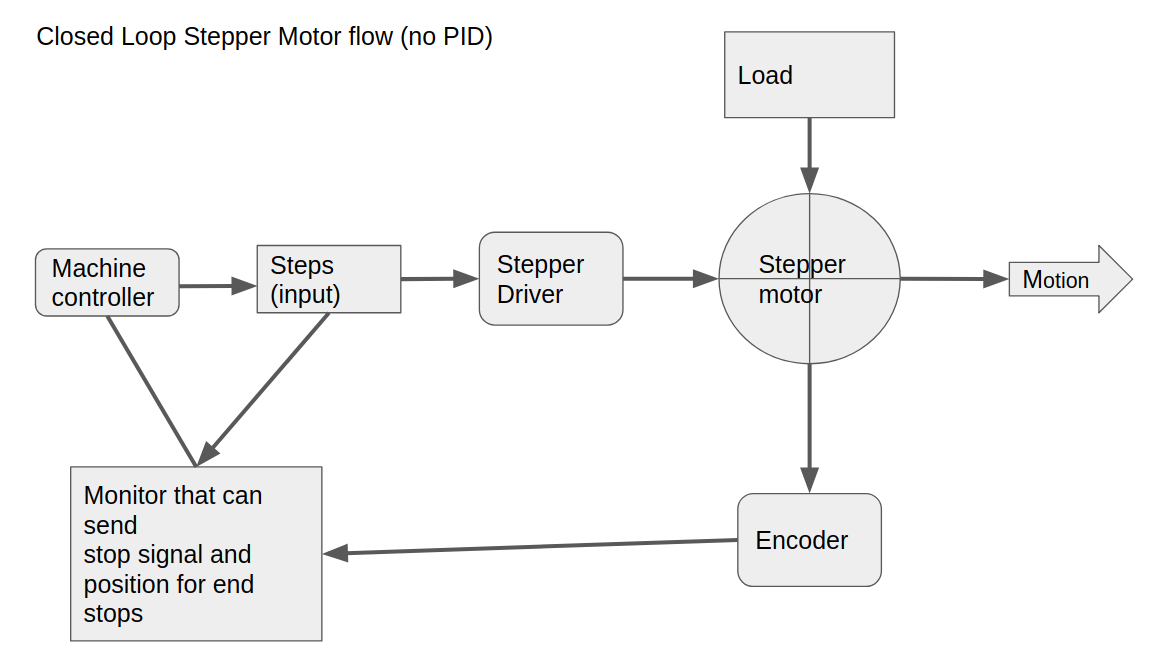
\includegraphics[width=0.8\textwidth]{CLSM_noPID.png}
  \captionsetup{justification=centering}
  \caption{Closed-Loop Stepper control flow with not feedback}
   \label{fig:CLSM}
\end{figure}
\par
The non-servo CLSM can use the encoder not only for end stops and error reporting but also to send correction steps from the motor controller to compensate for missed steps. 
\par
It should be noted that advanced type CLSM products such as StepSERVO™ from Applied Motion Products with full feedback servo control also have costs which are  comparable BLDC or AC servo systems and also require tuning just as conventional servos. It is unclear at this point what if any advantage such systems offer over equally priced competitors. 

%http://www.galilmc.com/news/servotrends-whats-new-galil/white-paper-forms-closed-loop-stepper-control
%\begin{displayquote}
%End-Point Correction
% By utilizing encoder feedback to recognize this position error, the end point can be adjusted by
%commanding additional step pulses to bring the motor into the correct position. Galil calls this Stepper
%Position Maintenance mode, or SPM
%\end{displayquote}
%https://www.mclennan.co.uk/news/comparing-open-loop-and-closed-loop-stepper-systems
%%AccuForce (yet another competitor doing more or less the same thing)
%https://simxperience.com/Community/SimXperienceDevelopersBlog/TabId/783/ArtMID/1674/ArticleID/28/Hybrid-Stepper-Servo-vs-Traditional-Stepper-vs-Traditional-Servo.aspx

\subsection{Servos}

For the purposes of this report a "servo" is an electrical motor, encoder and control system suitable for providing motion control based on an error correction feedback loop. (closed loop control system) This is customarily accomplished with the use of rotary encoders mounted on the drive motor but other solutions as possible such as linear encoders that measure movement relieving the system from the uncertainty of backlash and other errors when the motor is directly measured. The feedback is traditionally provided by a tuned Proportional Integral Derivative (PID) control algorithm.
\par
The motors are themselves similar to steppers although are more linear and lack the detent torque found with steppers. The main differentiating electromechanical component is the encoder which allows location determination to a much finer resolution than is possible with a hybrid stepper motor. Typical hybrid stepper motors have 200 steps per revolution (1.8 degrees). While microstepping does to some extent provide higher resolution it is not without its drawbacks and without actual feedback there is no way to ensure the accuracy is reached, even if it is theoretically possible. Microstepping is practically limited to around 10x which approximates 2000 steps per revolution which is the minimum resolution of most servo encoders. Practically servo resolution is only limited by budget and processing power. 
\par
There are three main ways to classify motors: by their current AC or DC; by the way in which they achieve commutation brushless or brushed; and by the average speed of their rotating field (rotor) synchronous or asynchronous.
\subsubsection{AC Servo}\label{acservo}
The traditional high-end servo option is to use an 3 phase AC induction motor. This provides the smoothest possible motion and it is possible to use resolvers to measure location rather than a physical encoder. Although in modern application the resolver is of less use it is not an option with permanent magnet DC motor based servos. All modern servos (AC or DC) are brushless although the drive mechanics are slightly different given back emf is a function of induction with the AC motors vs permanent magnet in BLDC motors. AC induction motors are by nature asynchronous while BLDC and Stepper Motors are synchronous, meaning the induced field and the rotor turn at the same average rate while induction motors must have a difference in speed between two rotor and applied field to produce torque. Unlike stepper motors, AC servos and control not just position but also torque, speed and other characteristics. Servos in general are more capable of handling peak loads and therefore must not be sized as large as a stepper motor in a comparable application. Not only can they correct if the applied loads exceed the applied power but it is also possible to overdrive a servo to considerably above the rated power for a short time. This is useful but just for peak loads but also means it is possible to achieve higher accelerations with a servo than a stepper of a similar size/capacity. 
\par
There are some drawbacks, the costs involved with an AC servo system are considerably more than with a traditional stepper system, even accounting for the more efficient motor use, but the optional performance of an AC servo is also much higher than a stepper. Part of this cost comes from the need for an encoder. Encoders, particularly high resolution and high speed units, are relatively expensive. The associated control electronics are also far more complex and require considerably more processing power than a stepper driver based motion control system. 

\subsubsection{Brushless DC Servo}
The other main category of modern servo motor is the Brushless DC motor, (BLDC) which like AC servos are 3phase but use permanent magnets rather than induction to induce the back EMF in the rotor. Early DC servos were made using brushed motors, these while more simple to control (as they use a physical commutator rather than an encoder computer based system) have generally fallen into disfavor do to the disadvantages of brushed motors and the cost and availability of brushless motors has improved. 
\par
While BLDC (Brushless DC) Servos and AC servos are physically both three phase brushless motors with encoders there are some significant differences. As mentioned in section in section \ref{acservo} synchronous permanent magnet motors they require electronic commutation and therefore must have encoders (even when used simply for power and not detailed motion control). BLDC motors have favorable properties in certain applications and are perhaps the best motor best motor of general purpose high performance servo development. 
\subsubsection{Brushed DC Servo}
Although not considered top level technology brushed DC servos still can have applications in modern control systems. They are less expensive, easier to control, smaller, and more efficient than BLDC or AC servos. The brushes wear but in applications with moderate use they can over a compelling options. Like AC servos they can be over-driven for higher torque or power than rated. 

\subsection{Control approaches}  
Feedback control systems are not limited to PID, there are other options which can offer improved performance in certain situations. Some of these approaches are not greatly dissimilar to those proposed by PolarWorks. These systems include: Linear Quadratic Gaussian (LQG) and Model Reference Adaptive Systems (MRAS).
\subsection{Motor Type discussion}

Motor selection needs to be based on the measured performance of the various options. There are at present there may be some misconceptions about motor properties, prices and availability. 

\par 
The authors can find no literature or simulation results that show stepper motors to be advantageous over other motors types when using encoders and full feedback. Either an AC induction motors or BLDC 3 phase motor would be more linear, easier to model mathematically given the absence of detent torque and other factors. The only known application where stepper motors are advantageous is when they may be used in as pure stepper motors without encoders etc. In certain specific (low end) applications the cost benefits of simple motor drives and the lack of expensive encoders make steppers a viable option. Stepper motors however do not appear to be the ideal platform for a feedback based servo system.
\par 
The cost difference of the motor for a BLDC vs a Stepper is not a significant. BLDC motors are widely available from both low cost (China) and high quality (Swiss/German) sources for prices which are similar to stepper motors from equivalent sources. In terms of manufacturing complexity a stepper motor is actually more demanding so given similar volume of production a conventional BLDC motor should actually be less expensive to produce than an equivalent size stepper motor. This negation of the supposed cost advantage of stepper motors is further eroded by the higher efficiency and overdrive potential of BLDC motors which may therefore be sized smaller than a stepper in an identical application. 
\par
When comparing conventionally driven stepper motors with full servo feedback systems there are differences in performance which are not obvious if simply step or microstep is compared to encoder resolution. Stepper motors (running steps) are inherently less accurate than closed loop servos. \footnote{page 320 Electric Motors and Drives 2006}
\begin{quote}
In the previous discussion the load torque was assumed to be zero, and the rotor was therefore able to come to rest with its poles exactly in line with the excited stator poles. When load torque is present, however, the rotor will not be able to pull fully into alignment, and a 'step position error' will be unavoidable
\end{quote}
This means that without an encoder a stepper in a real application (one with load), it is likely that a stepper will be less accurate than the theoretical step (microstep) size. 
\section{Simulation}
As an evaluation of the relative performance and to identify areas of particular suitability a simulation was conducted. This simulation models the control system performance for .... 

\begin{figure}[h!]
  \centering
  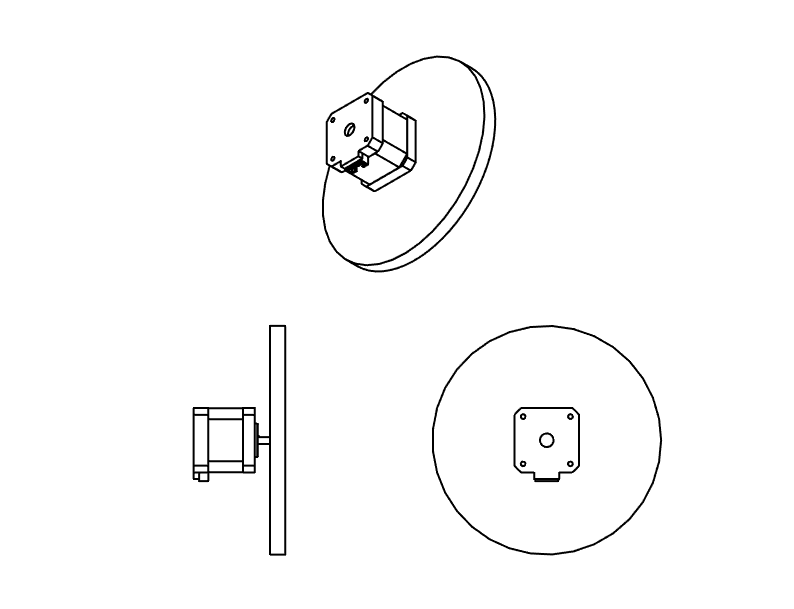
\includegraphics[width=0.8\textwidth]{simulation.png}
  \captionsetup{justification=centering}
  \caption{Rotor configuration for Simulation}
   \label{fig:sim}
\end{figure}
\subsection{PolarDrive}
We implemented the inverse approach ... At an angular acceleration rate $\alpha=100$ we find nearly perfect and smooth tracking along the motion path in Figure \ref{fig:hyb-alpha-100}
\begin{figure}[h!]
  \centering
  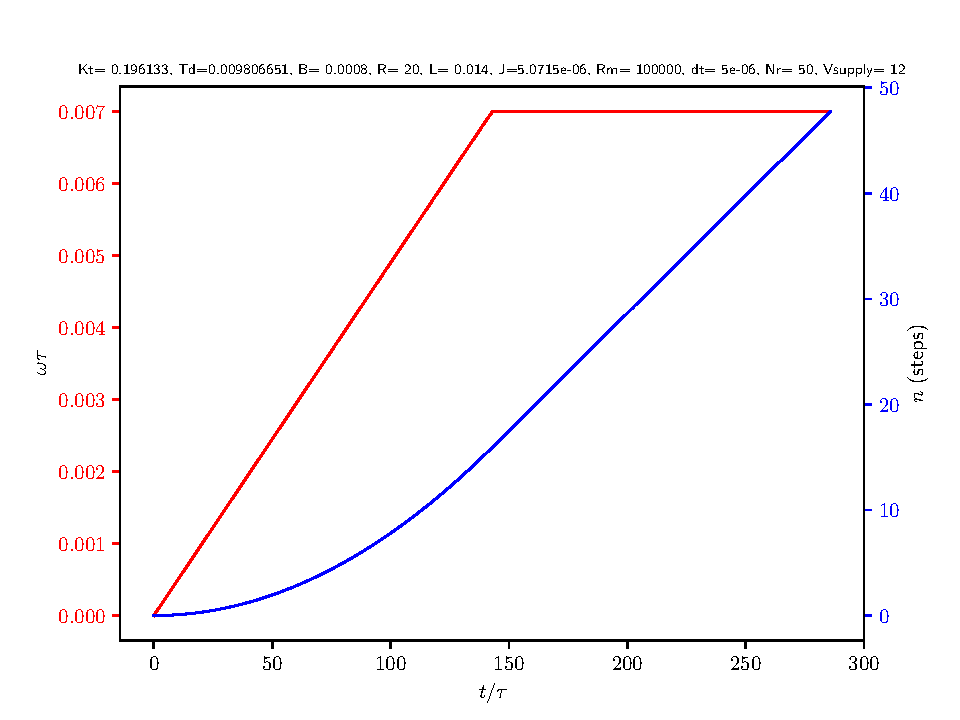
\includegraphics[width=0.9\textwidth]{simfigs/fig1-2018-10-20T14-13-59-hybrid-accel-False-alpha-100.pdf}
  \captionsetup{justification=centering}
  \caption{The inverse scheme at $\alpha=100$}
   \label{fig:hyb-alpha-100}
\end{figure}
We then tested the this inverse scheme at $\alpha=460$ and higher in Figures \ref{fig:hyb-alpha-460} and \ref{fig:hyb-alpha-500}. 
\begin{figure}[h!]
  \centering
  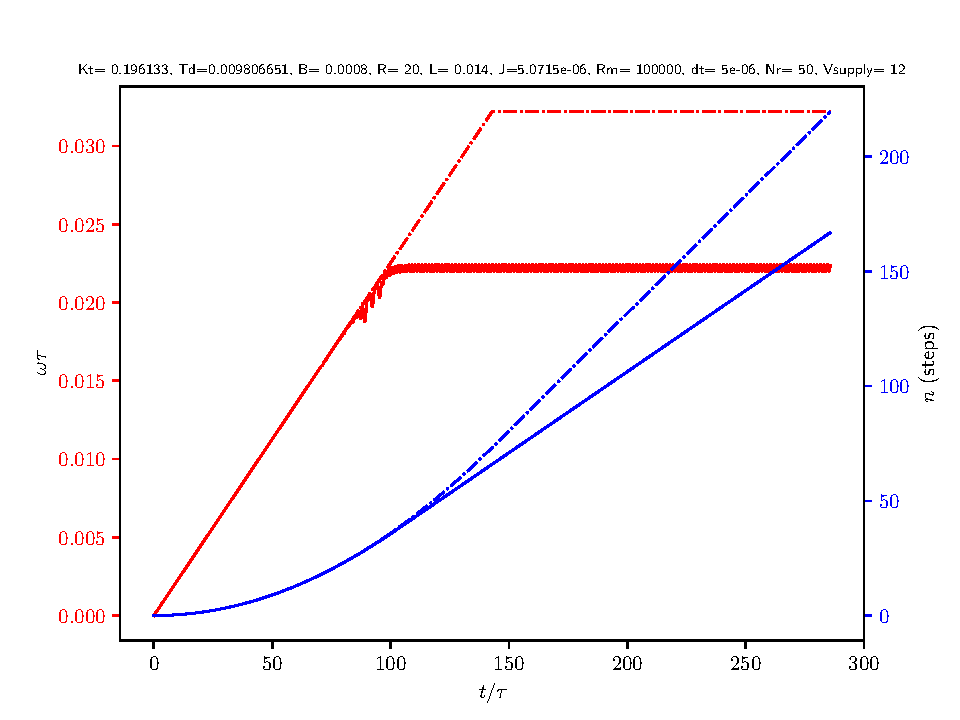
\includegraphics[width=0.9\textwidth]{simfigs/fig1-2018-10-20T14-24-16-hybrid-accel-False-alpha-460.pdf}
  \captionsetup{justification=centering}
  \caption{The inverse scheme at $\alpha=460$}
   \label{fig:hyb-alpha-460}
\end{figure}

\begin{figure}[h!]
  \centering
  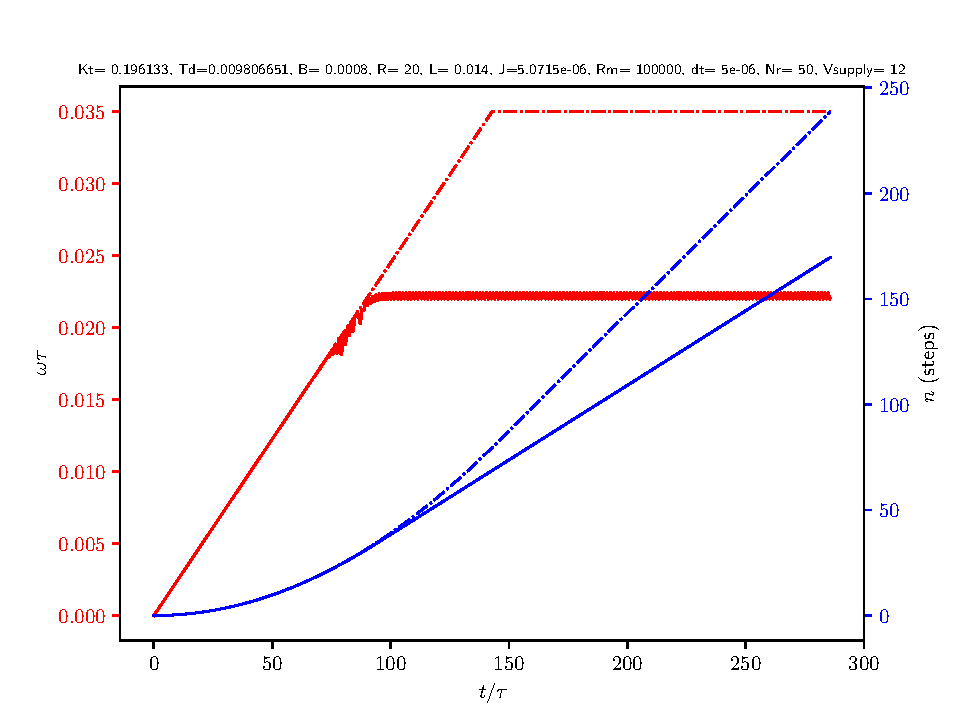
\includegraphics[width=0.9\textwidth]{simfigs/fig1-2018-10-20T14-36-07-hybrid-accel-False-alpha-500.pdf}
  \captionsetup{justification=centering}
  \caption{The inverse scheme at $\alpha=500$}
   \label{fig:hyb-alpha-500}
\end{figure}
We also have a separate inverse scheme that precomputes the coil excitations once before runtime, shown in Figure \ref{fig:rev-alpha-500}

\begin{figure}[h!]
  \centering
  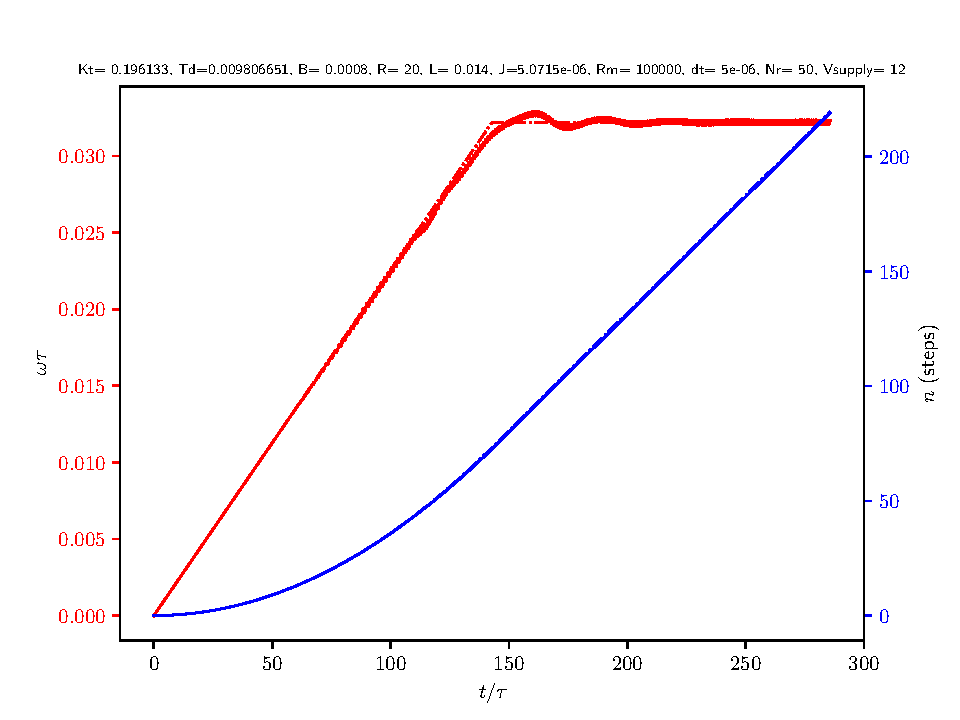
\includegraphics[width=0.9\textwidth]{simfigs/fig1-2018-10-20T14-23-39-reverse-alpha-460.pdf}
  \captionsetup{justification=centering}
  \caption{The reverse inverse scheme at $\alpha=460$}
   \label{fig:rev-alpha-460}
\end{figure}

\begin{figure}[h!]
  \centering
  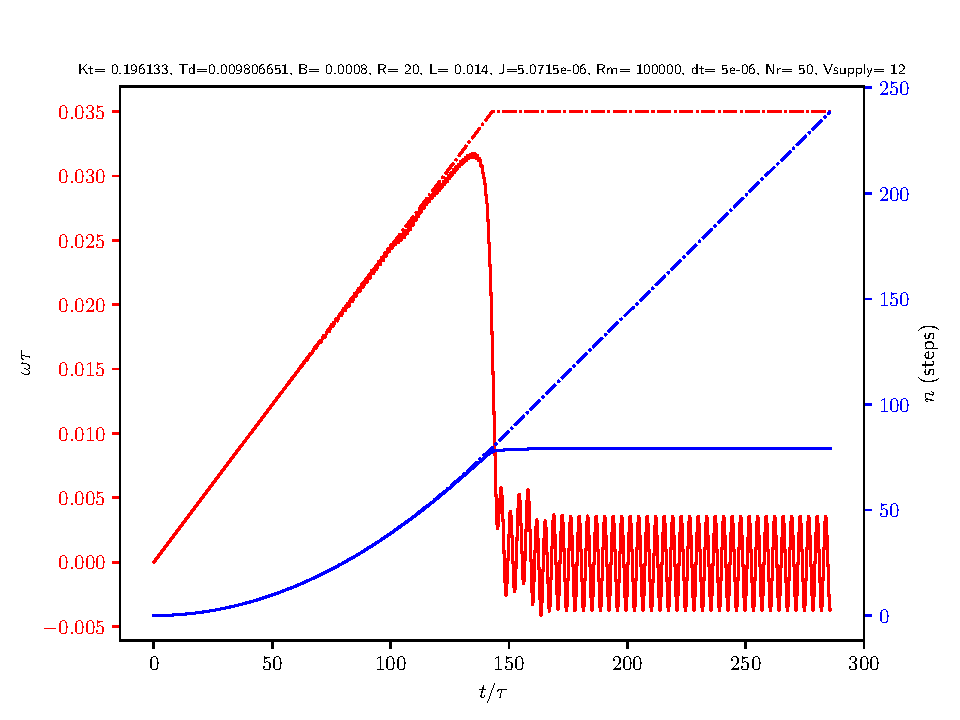
\includegraphics[width=0.9\textwidth]{simfigs/fig1-2018-10-20T14-37-59-reverse-alpha-500.pdf}
  \captionsetup{justification=centering}
  \caption{The reverse inverse scheme at $\alpha=500$}
   \label{fig:rev-alpha-500}
\end{figure}

\subsection{Driven Hybrid Stepper Motor}
For comparison with the PolarDrive inverse approach we first chose a single step hybrid stepper motor. We chose high angular acceleration rate $\alpha$ and found in Figure \ref{fig:step-alpha-100}

\begin{figure}[h!]
  \centering
  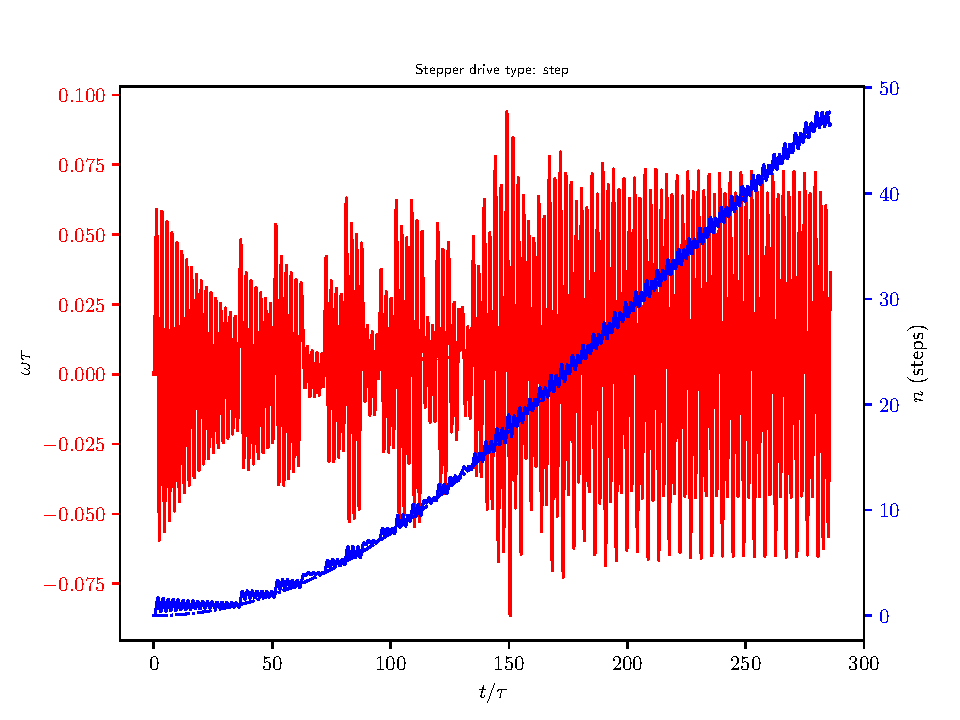
\includegraphics[width=0.9\textwidth]{simfigs/fig1-2018-10-20T14-16-17-step-alpha-100.pdf}
  \captionsetup{justification=centering}
  \caption{Microstepping at higher $\alpha$}
   \label{fig:step-alpha-100}
\end{figure}

\begin{figure}[h!]
  \centering
  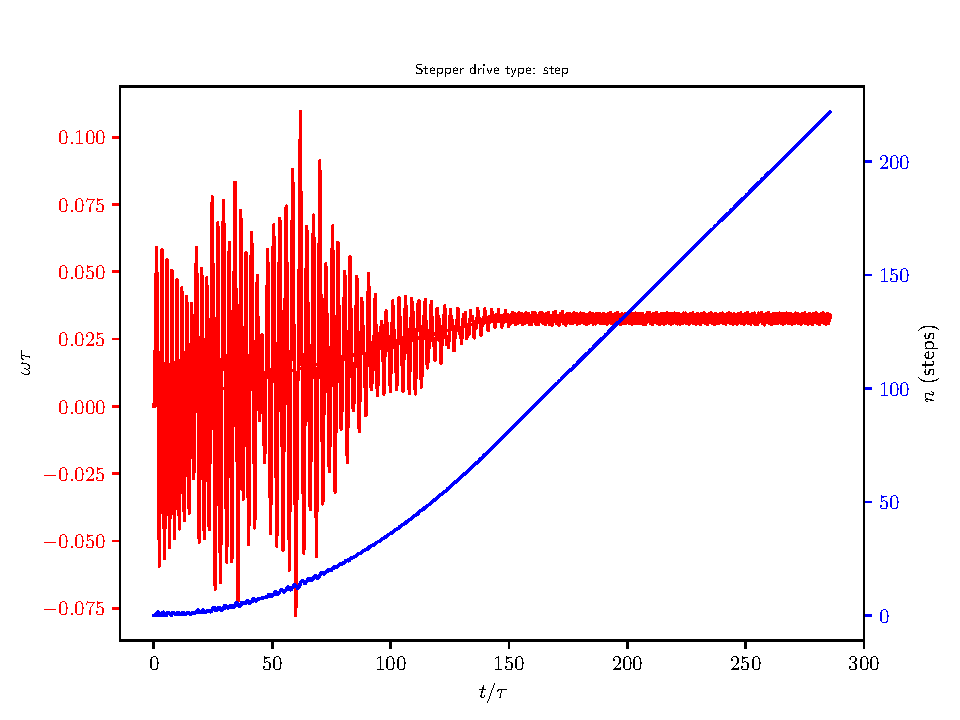
\includegraphics[width=0.9\textwidth]{simfigs/fig1-2018-10-20T14-29-43-step-alpha-465.pdf}
  \captionsetup{justification=centering}
  \caption{Microstepping at higher $\alpha=465$}
   \label{fig:step-alpha-465}
\end{figure}

\subsection{Microstepping Hybrid Stepper Motor}
For smoothness, microstepping is often used. At $\alpha=100$ we find the behavior in Figure \ref{fig:micro8-alpha-100}.
\begin{figure}[h!]
  \centering
  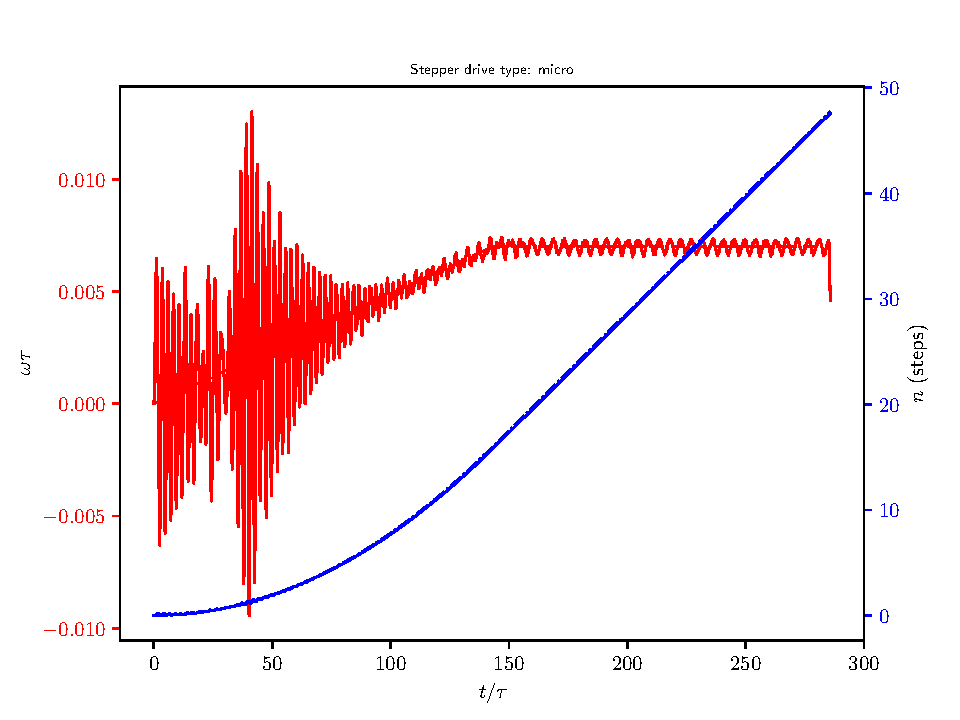
\includegraphics[width=0.9\textwidth]{simfigs/fig1-2018-10-20T14-18-54-micro8-alpha-100.pdf}
  \captionsetup{justification=centering}
  \caption{Microstepping at $\alpha=100$}
   \label{fig:micro8-alpha-100}
\end{figure}
We also simulated microstepping ... at high angular acceleration we find in Figure \ref{fig:micro8-alpha-465} and Figure \ref{fig:micro8-alpha-500}.
\begin{figure}[h!]
  \centering
  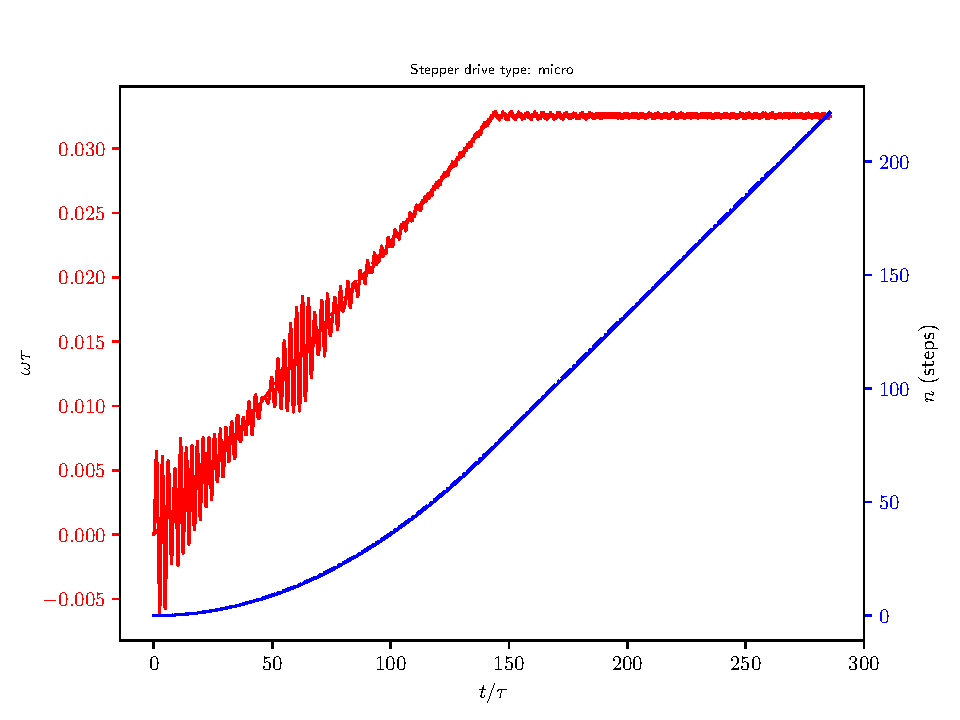
\includegraphics[width=0.9\textwidth]{simfigs/fig1-2018-10-20T14-32-16-micro8-alpha-465.pdf}
  \captionsetup{justification=centering}
  \caption{Microstepping at higher $\alpha = 465$}
   \label{fig:micro8-alpha-465}
\end{figure}

\begin{figure}[h!]
  \centering
  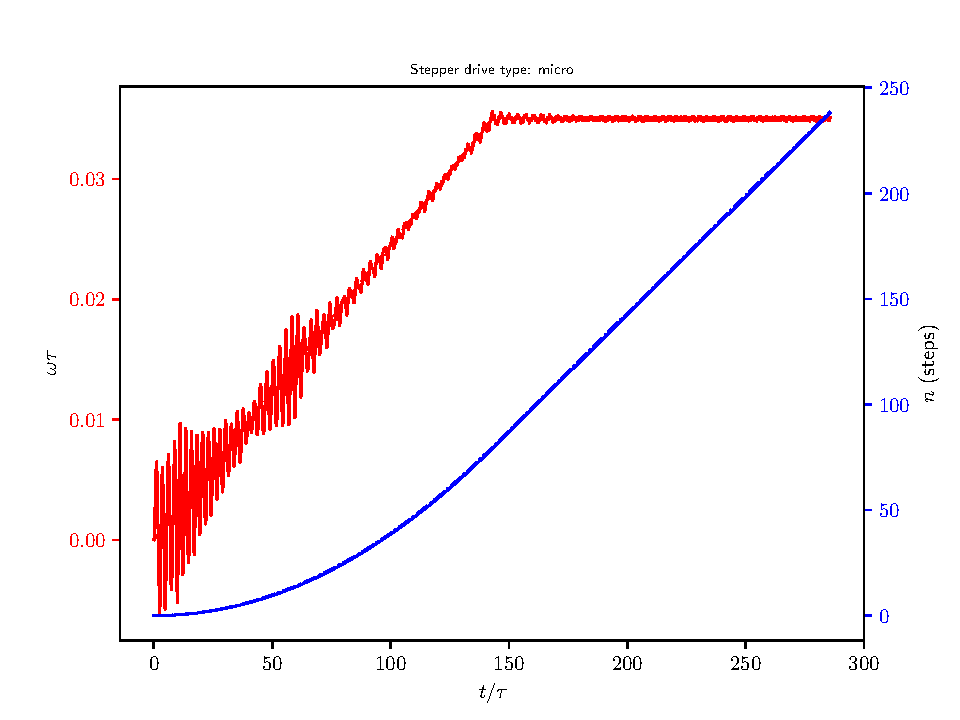
\includegraphics[width=0.9\textwidth]{simfigs/fig1-2018-10-20T14-34-21-micro8-alpha-500.pdf}
  \captionsetup{justification=centering}
  \caption{Microstepping at higher $\alpha = 500$}
   \label{fig:micro8-alpha-500}
\end{figure}
\subsection{Closed Loop Stepper Motor}
Although the original intention was to simulate the performance of a stepper motor driven via PID feedback, it was identified during the literature search that such an approach was well covered and did not require further simulation by PolarWorks. In the paper Adaptive PID control of a stepper motor driving a flexible rotor from Nehal M. Elsodany et all\footnote{Alexandria University,
Alexandria Engineering Journal, 30 August 2011} 

\section{Conclusion}
\subsection{Comparison of PolarDrive vs other systems via simulation}
This will be done, at least initially by means of mathematical simulation. A simulation of the performance of the current PolarDrive system will be compared with three other simulations of the same single axis rotor following identical acceleration paths.

We can evaluate the limiting behavior of our inverse approach vs microstepping by examining the excitations and $\delta$ for each of the drive schemes for $alpha=500$ in Figure \ref{fig:exc-hyb-alpha-500}, \ref{fig:exc-rev-alpha-500}, and \ref{fig:exc-micro-alpha-500} for the excitations, while $\delta$ for the inverse schemes is shown in Figure \ref{fig:delta-hybrid-alpha-500} and \ref{fig:delta-rev-alpha-500}
\begin{figure}[h!]
  \centering
  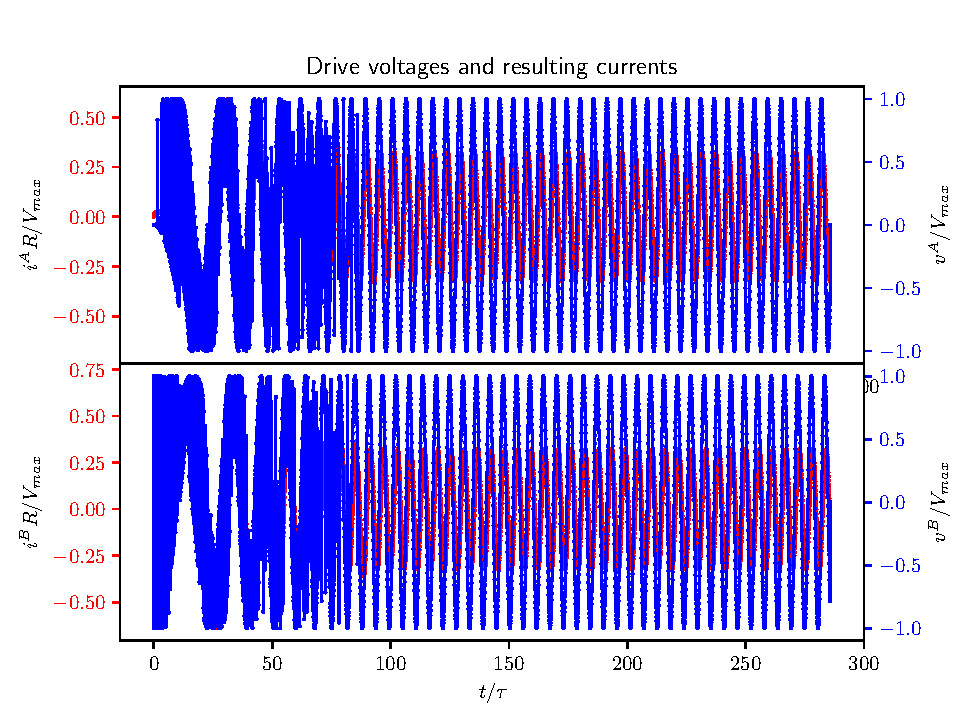
\includegraphics[width=0.9\textwidth]{simfigs/fig3-2018-10-20T14-36-07-hybrid-accel-False-alpha-500.pdf}
  \captionsetup{justification=centering}
  \caption{The excitation for the hybrid inverse scheme at $\alpha=500$}
   \label{fig:exc-hyb-alpha-500}
\end{figure}
\begin{figure}[h!]
  \centering
  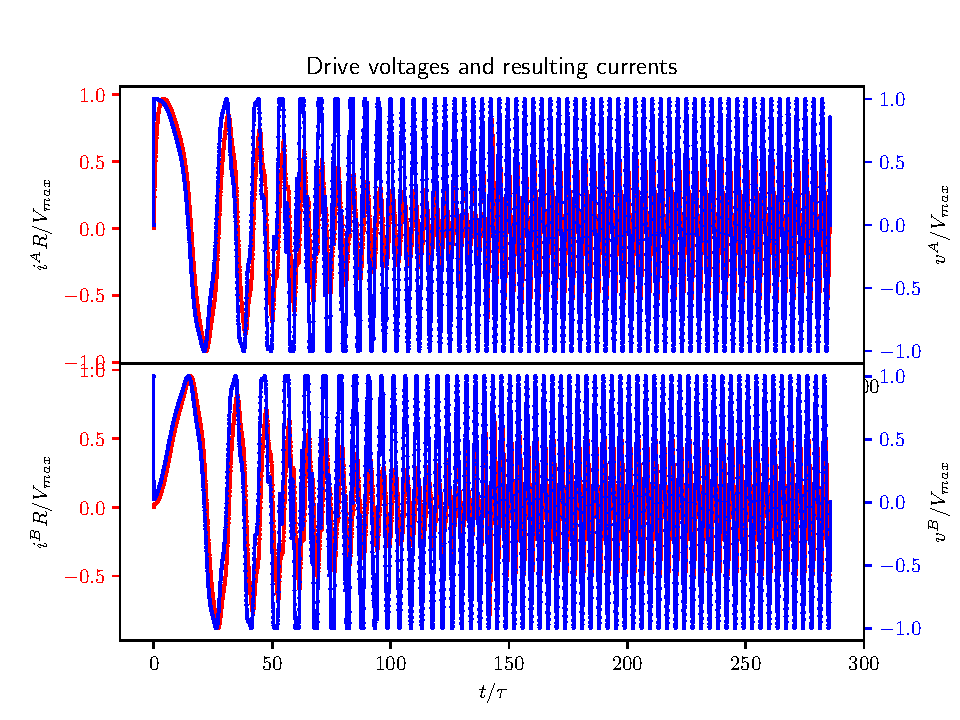
\includegraphics[width=0.9\textwidth]{simfigs/fig3-2018-10-20T14-37-59-reverse-alpha-500.pdf}
  \captionsetup{justification=centering}
  \caption{The excitation for the reverse inverse scheme at $\alpha=500$}
   \label{fig:exc-rev-alpha-500}
\end{figure}
\begin{figure}[h!]
  \centering
  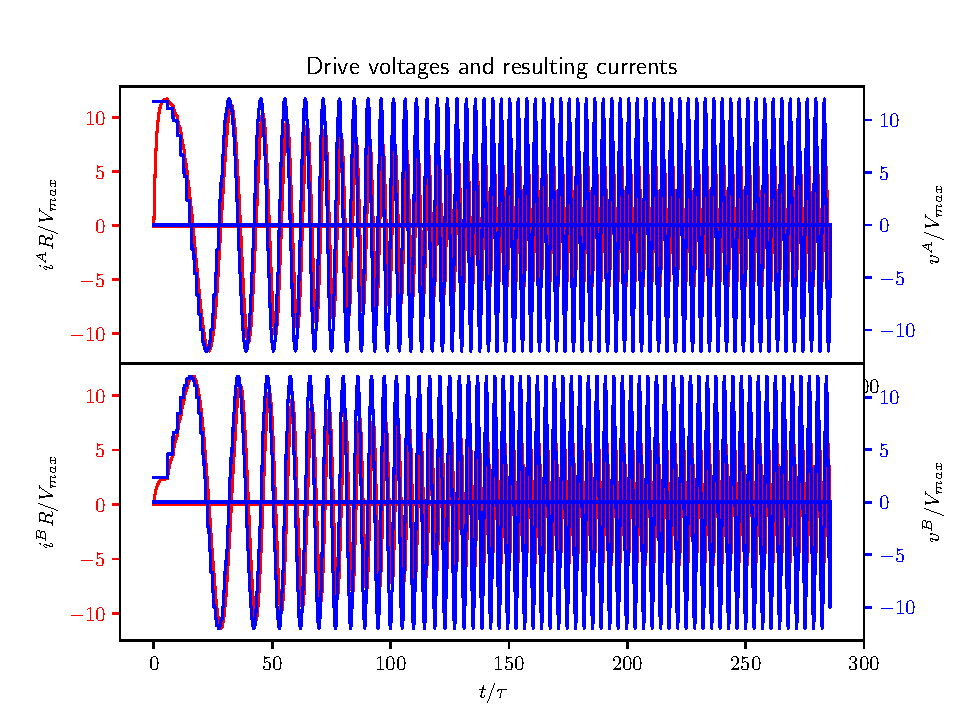
\includegraphics[width=0.9\textwidth]{simfigs/fig3-2018-10-20T14-34-21-micro8-alpha-500.pdf}
  \captionsetup{justification=centering}
  \caption{The excitation for the microstepping 8 scheme at $\alpha=500$}
   \label{fig:exc-micro-alpha-500}
\end{figure}
\begin{figure}[h!]
  \centering
  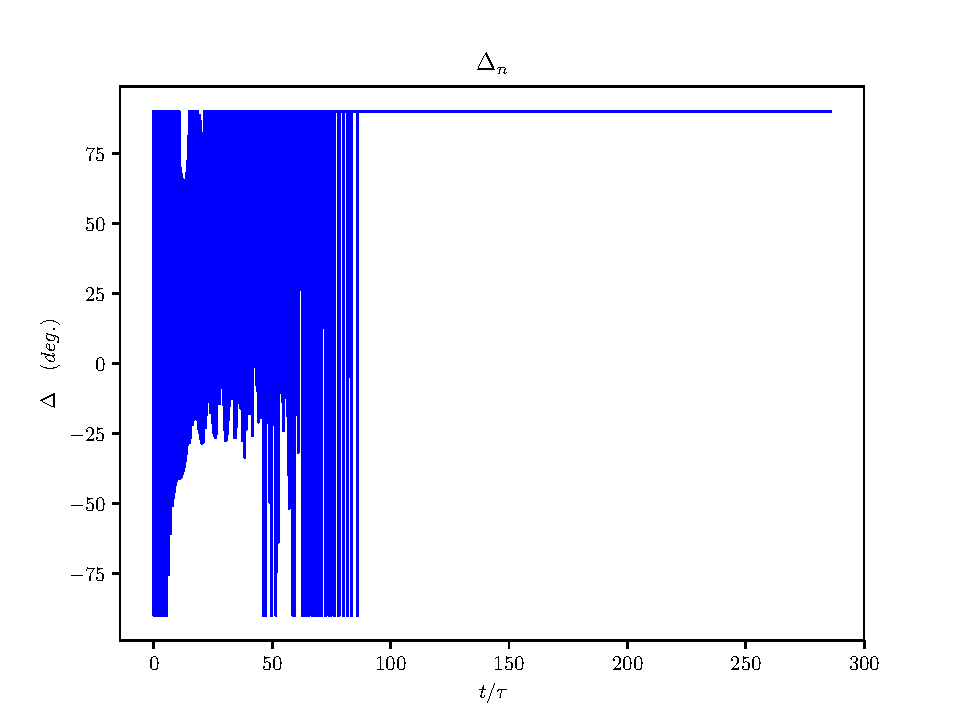
\includegraphics[width=0.9\textwidth]{simfigs/fig5-2018-10-20T14-36-07-hybrid-accel-False-alpha-500.pdf}
  \captionsetup{justification=centering}
  \caption{$\delta$ for the hybrid inverse scheme at $\alpha=500$}
   \label{fig:delta-hybrid-alpha-500}
\end{figure}
\begin{figure}[h!]
  \centering
  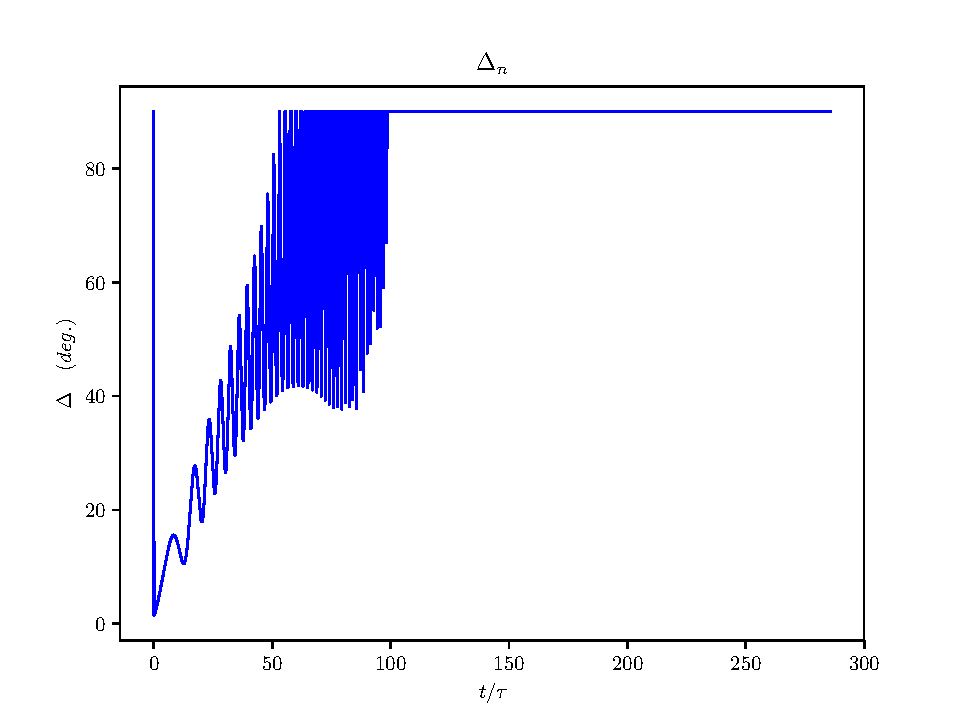
\includegraphics[width=0.9\textwidth]{simfigs/fig5-2018-10-20T14-37-59-reverse-alpha-500.pdf}
  \captionsetup{justification=centering}
  \caption{$\delta$ for the reverse inverse scheme at $\alpha=500$}
   \label{fig:delta-rev-alpha-500}
\end{figure}

\subsection{PolarDrive Performance evaluation General Discussion}
how does it compare, what is it good at, where do we need to do more work, what about the current implementation should be reevaluated. 
   
\subsection{Supporting system evaluation}
The opportunities offered by Step-NC are considerable and it appears, at least technically, that the wide scale implementation of STEP-NC from CAD software through the entire manufacturing process is completely viable. Step-NC or similar MBD approaches have been used corporations such as Boeing Commercial Airplanes for over a decade and given the widespread adaption of 3D cad in all levels of industry it is a logical progression. \par 
Given that there are many non-experts designers who lack the training or experience to understand Geometric Dimensioning and Tolerancing, properly developed fully integrated CAM software could be helpful in identifying problems and driving design changes before going to manufacturing. The preservation of the model as a 3D solid rather than a paths created from a point cloud as is currently done using conventional G-code would be advantageous, not only in creating more faithful machine paths but also in post production inspection and other quality control. This becomes even more important with additive manufacturing and other evolving technologies. 



\section*{Additional material to be removed}

Internal performance analysis report (Target completion: August 
\begin{itemize}
\item Control algorithm analysis report (Target completion: June 2018):
i. Does the control algorithm analysis test the performance of the
Polarworks approach against, at a minimum, three other alternative
approaches? Y/N?
\item 
Does the control algorithm analysis summarize the findings of those tests
such that third party (propose a member of the board) can understand
the implications and results of the test? Y/N?
\item Does the control algorithm analysis report clearly outline the
strengths and weaknesses of Polarworks’ approach against the
alternatives such that decisions can be made regarding its competitive
advantage or ability to disrupt in proposed markets? Y/N?

\end{itemize}

\begin{appendix}

\section{Equations of motion}
Back EMF for coil A and B respectively are calculated as:
\begin{equation}\label{e_A}
	e_A = -K_m \omega \sin(N_r\theta)
\end{equation}
\begin{equation}\label{e_B}
	e_B = K_m \omega \cos(N_r\theta)
\end{equation}
\\
The rate-of-change of the current for the coils are:
\begin{equation}\label{di_A}
	\frac{di_A}{dt} = (v_A(t) - R i_A - e_A ) / L
\end{equation}
\begin{equation}\label{di_B}
	\frac{di_B}{dt} = (v_B(t) - R i_B - e_B ) / L
\end{equation}
\\
Acceleration, angular velocity, friction and torque are related as:
\begin{equation}\label{acceleration}
	J \frac{d \omega}{dt} + B \omega = T_e
\end{equation}
\\
The Torque term equates to:
\begin{equation}\label{torque}
	T_e = 	- K_t \left(i_A - \frac{e_A}{R_m}\right)\sin(N_r\theta)	
	 		+ K_t \left(i_B - \frac{e_B}{R_m}\right) \cos(N_r\theta)
	 		- T_d\sin(4N_r\theta)
\end{equation}
\\
To complete the set of differential equations we have the derivative of $\theta$ 
\begin{equation}\label{mathworks:velocity}
	\frac{d\theta}{dt} = \omega
\end{equation}
\section{Non-dimensionalization}
We can non-dimensionalize the equations to discover the important grouping of terms. To this end we scale all the variables as follows
\begin{subequations}
\begin{align}
t &= \frac{L}{R} \hat{t}\\
\frac{d\phantom{t}}{dt} &= \frac{R}{L} \frac{d\phantom{t}}{d\hat{t}}\\
e^A &= V_{max} \hat{e}^{A}\\
e^B &= V_{max} \hat{e}^{B}\\
v^A &= V_{max} \hat{v}^A\\
v^B &= V_{max} \hat{v}^B\\
i^A&= \frac{V_{max}}{R} \hat{i}^A\\
i^B&= \frac{V_{max}}{R} \hat{i}^B\\
\omega &= \frac{R}{L} \hat{\omega}
\end{align}
\end{subequations}
With these scalings the equations read
\begin{subequations}
\begin{align}
e_A =& - C_4 \omega \sin(N_r\theta)\\
e_B =& + C_4 \omega \cos(N_r\theta) \\
\frac{di^A}{dt^{\ }} =& v^A(t) -  i^A - e^A \\
\frac{di^B}{dt^{\ }} =& v^B(t) -  i^B - e^B \\
\frac{d\theta}{dt} =& \omega\\
C_1 \frac{d \omega}{dt} + (C_2+ C_4 \frac{R}{R_m}) \omega =& 	- i_A \sin(N_r\theta)	+ i_B \cos(N_r\theta)- C_3 \sin(4N_r\theta) 
\end{align}
\end{subequations}
where the non-dimensional constants $C_i$ are 
\begin{subequations}
\begin{align}
C_1 = & \frac{J R^3}{K_t V_{max} L^2}\\
C_2 = & \frac{R^2\beta}{K_t V_{max} L}\\
C_3 = & \frac{T_d R}{K_t V_{max}}\\
C_4 = & \frac{K_t R}{V_{max} L}
\end{align}
\end{subequations}

Alternatively, we can scale $\omega$ {\it or} $\alpha = d\omega/dt$ by the maximum values the motor torque could produce, that is
\begin{align}
\alpha \equiv& \frac{d\omega}{dt} = \frac{V_{max} K_t}{R \, J} \alpha\\
\omega \equiv& \frac{d\theta}{dt} = \frac{V_{max} K_t}{R \, B} \omega
\end{align}


\section{Statement of inverse problem}
Given a specified motion $\theta(t), \dot\theta(t)$,  can we find $v_A(t)$ and $v_B(t)$ that produce these motions for acceptable values of $i_A(t) $ and $i_B(t)$? Substituting \vsol into the above equations should then forward-integrate to provide the desired \thetasol. Similarly, if we substitute \thetasol and \vsol into the equations we should get an identity.

Since both currents show up in the torque equation, we might imagine a whole class of solutions to the inverse problem. For example, with a gentle enough motion, energizing just one or the other coil might reproduced the desire motion. 

In addition to the possibility of multi-valued solutions, we might expect that physical considerations might preclude any theoretical inverse. For example, we might be asking for more voltage or current than the supply can deliver or that the coils can handle. We will address such constraints later. 

\section{A succession of more complicated inverse problems}
Consider the forced harmonic oscillator
\begin{equation}
m \ddot x + b \dot x + k x = f(t)
\end{equation}
If we specify a twice-differentiable function $x'(t)$ as the desired motion, for example, $x'(t) = v_0 t + x_0$, then we find the control function is 
\begin{equation}
f(t) = m \ddot x'(t) + b \dot x'(t) + k x'(t) = b v_0 + k v_0 t + k x_0
\end{equation}
Now suppose that the forcing function obeys its own dynamic, for example
\begin{align}
\frac{df}{dt} + f(t) / \tau = V(t) \\
m \ddot x + b \dot x + k x = f(t) 
\end{align}
Then $f(t)$ is still as in (9), but now we need to determine the control input function $V(t)$. Then (10) becomes
\begin{equation}
V(t) = k v_0 + ( b v_0 + k v_0 t + k x_0)/\tau
\end{equation}
Now consider that there are two forces acting on the mass-spring system
\begin{align}
\frac{df_1}{dt} + f_1(t) / \tau = V_1(t)\\
\frac{df_2}{dt} + f_2(t) / \tau = V_2(t)\\
m \ddot x + b \dot x + k x = f_1(t) + f_2(t)
\end{align}
Now it is not possible to uniquely find $V_1, V_2$. (13) and (14) can be solved for $f_1, f_2$ in terms of integrals over $V_1, V_2$, but then (15) is not sufficient in itself to pick out a unqiue solution.

Clearly, for these kinds of problems we need auxillary conditions to lock down unique solutions, or else we must utilize the freedom in (15) in order to generate some inversion algorithm albeit a non-unique solution. 

\section{Solution of inverse problem}
\subsection{Closed form solutions}
If we were specified functional forms for the desired motion we might be able to immediately identify \vsol algebraically. For example, lets assume we want $\theta(t)= \Omega t,\, \dot\theta=\Omega$. Substitution yields the set of equations
\begin{align}
\frac{di_A}{dt} + i_A / (L/R) &= (v_A(t) + K_m \Omega \sin(N_r\Omega t) ) / L\\
\frac{di_B}{dt} + i_B / (L/R) &= (v_B(t) - K_m \Omega \cos(N_r\Omega t) ) / L
\end{align}
and 
\begin{equation}
\begin{split}
- K_m \left(i_A + \frac{K_m \Omega \sin(N_r\Omega t)}{R_m}\right)\sin(N_r\Omega t) 
	 		&+ K_m \left(i_B - \frac{K_m \Omega \cos(N_r\Omega t)}{R_m}\right) \cos(N_r\Omega t)\\
	 		&- T_d\sin(4N_r\Omega t) - B \Omega\\ & = 0
\end{split}	 		
\end{equation}	
The equations for the two currents can then be solved by quadrature, that is, \isol would be defined in terms of integrals of \vsol over time. The resulting forms for the two currents could be substituted back into the torque balance equation. Thus, to solve for \vsol, we need to solve an equation of the form \begin{equation}
F_1(v_A(t), t) + F_2(v_B(t), t) + F \equiv 0
\end{equation}
for \vsol; this gives us an integral equation for \vsol, a  Herculean task on its face even for the simplest form of proposal motion. However, we may be able to use this idea in the sequel. We can also examine rotating \vsol\ idea, I believe there is some connection to this type of special solution.  

\subsection{Approximate solutions by linearization, discretization, and perturbing off equilibrium solutions}
\subsubsection{Linearization}
Several articles pointed to by Jakob hint at a linearization scheme. We can examine this approach in the context of finding \vsol at time $t+\Delta t$ given values of all the variables at time $t$. In this case we can expand all nonlinear functions about their values at time $t$

\subsubsection{Discretization}
Related to linearization, we can use Euler and or other methods for solving differential equations, with the twist that we start with the discretized form of the solution and work backwards to \vsol. 

For example, let $t = n \Delta t$, $\theta_n \equiv \theta(n \Delta t)$  be given. We take $\omega_n = (\theta_{n+1} - \theta_n)/\Delta t$. Let 
\begin{align}	
e^A_n &= -K_m \omega_n \sin(N_r \theta_n)\label{discreteeA}\\
e^B_n &= \phantom{-}K_m \omega_n \cos(N_r \theta_n)\label{discreteeB}
\end{align}
then the currents in the coils are determined by
\begin{align}
\frac{i_{n+1}^A - {i_n^A}}{\Delta t} &= (v^A_{n+1}- R i_n^A - e^A_n)/L \label{discreteiA}\\
\frac{i_{n+1}^B - {i_n^B}}{\Delta t} &= (v^B_{n+1}- R i_n^B - e^B_n)/L \label{discreteiB}
\end{align}
and the torque requirement is
\begin{equation}\label{discreteT}
\begin{split}
J \frac{\omega_{n+1}-\omega_n}{\Delta t} + B \omega_n =& -K_m \left(i^A_{n+1} - \frac{e^A_n}{R_m}\right) \sin(N_r\theta_n) + K_m \left(i^B_{n+1} - \frac{e^B_n}{R_m}\right)\cos(N_r\theta_n)\\
 &- T_d \sin(4N_r\theta_n)
\end{split}
\end{equation}
We now need a scheme for first solving (\ref{discreteT}) for $i^{A,B}_{n+1}$, and then substituting the later currents into (\ref{discreteiA}) and (\ref{discreteiB}) to solve for $v^{A,B}_{n+1}$. 

can go forward in currents, leaving vs at later, substitute into torque, solve for vs. 

$T_d = 0$ gives a nice solution for slowly rotating fields. 

To lock down a unique solution, we might ask that the power input to the system be a minimum, so for example, $\min(v^A\cdot i^A + v^B\cdot i^B$). 

\subsubsection{Lead angle solutions}
A standard way of driving the stepper motor is with the assumption that the magnetic fields should lead ahead of the rotor position by some angle so as to apply torque of just the right amount. One issue here is that \vsol does not determine torques directly but only as they codetermine the currents in the coils.  By locking the two voltages together with a single lead angle, we loose the non-uniqueness of the inverse. However we sacrifice potential solutions for a given motion that do not satisfy this condition to some degree of approximation. 

Let us look at conditions under which the following voltages determine some specific form of rotary motion:
\begin{align}
V_t^A &= V^{\rm max} \cos(N_r \theta_t+\Delta_t)\\
V_t^B &= V^{\rm max} \sin(N_r \theta_t+\Delta_t)
\end{align}
where $\Delta$ is a slowly varying lead angle about the desired rotor position. We can then inquire under what conditions do coil excitations of this form lead to desirable rotor motion, and in what ways can we perturb off this solution to obtain a more general stepper motor rotor control scheme. 

First, we run this forward to see what steady state solutions are produced, trying $\theta(t) = \Omega t$ and $\Delta(t) = \Delta_0$. 

The rate-of-change of the current for the coils is now:
\begin{align}
\frac{di_A}{dt} &= (V^{\rm max} \cos(N_r \Omega t+\Delta_0) - R i_A + K_m \Omega \sin(N_r\Omega t) ) / L \\
\frac{di_B}{dt} &= ( V^{\rm max} \sin(N_r \Omega t +\Delta_0) - R i_B - K_m \Omega \cos(N_r\Omega t)  ) / L
\end{align}
If we wait a few time constants $L/R$ then we need only look at the particular solution. Of note is that the two currents are completely determined in terms of a constant $\Delta_0$. It remains to see if we can choose the offset in order to satisfy the torque condition (\ref{torque}). The solutions are:
\begin{align}
i_A &= c_1 e^{-\frac{R t}{L}}
+ \frac{K_m \Omega}{R \sqrt{\tau_L^2 N_r^2 \Omega ^2+1}}  \sin (N_r  \Omega t - \phi)
+ \frac{  V_{max}}{R  \sqrt{\tau_L^2 N_r^2 \Omega ^2+1} }  \cos (N_r \Omega t + \Delta_0 -\phi )  \\
i_B&=c_2 e^{-\frac{R t}{L}}
-  \frac{K_m \Omega}{R  \sqrt{\tau_L^2 N_r^2 \Omega ^2+1}} \cos ( N_r   \Omega t -\phi) 
+  \frac{V_{max}}{R \sqrt{\tau_L^2 N_r^2 \Omega ^2+1}}  \sin (N_r \Omega t + \Delta_0-\phi )
\end{align}
where $\phi = \tan^{-1}(\tau_L N_r \Omega)$. Now the torque balance condition (\ref{torque}) reads
\begin{equation}
\begin{split}
&-K_m \left(\frac{K_m \Omega}{R \sqrt{\tau_L^2 N_r^2 \Omega ^2+1}}  \sin (N_r  \Omega t - \phi)
+ \frac{  V_{max}}{R  \sqrt{\tau_L^2 N_r^2 \Omega ^2+1} }  \cos (N_r \Omega t + \Delta_0 -\phi )  + \frac{K_m \Omega \sin(N_r\Omega t)}{R_m}\right)\sin(N_r\Omega t) \\
&+ K_m \left(-  \frac{K_m \Omega}{R  \sqrt{\tau_L^2 N_r^2 \Omega ^2+1}} \cos ( N_r   \Omega t -\phi) 
+  \frac{V_{max}}{R \sqrt{\tau_L^2 N_r^2 \Omega ^2+1}}  \sin (N_r \Omega t + \Delta_0-\phi ) - \frac{K_m \Omega \cos(N_r\Omega t)}{R_m}\right) \cos(N_r\Omega t)\\
&- T_d\sin(4N_r\Omega t) - B \Omega\\ & = 0
\end{split}	 		
\end{equation}	
assuming the transient has decayed.  It is clear that at best $\Delta_0$ can be chosen to only approximately satisfy this condition. 

The same steps can be taken to deal with constant acceleration, $\theta_t = \frac{1}{2} \alpha t^2 + \Omega_0 t $ which gives an even more complicated condition for $\Delta_0$. 

\subsubsection{Discrete lead angle solutions}
Let us thus examine a discrete version of this same problem using the algorithm of (\ref{discreteeA})-(\ref{discreteT}). The applied voltages could be written as
\begin{align}
V_{n}^A &= V^{\rm max} \cos(N_r \theta_{n}+\Delta_{n})\\
V_{n}^B &= V^{\rm max} \sin(N_r \theta_{n}+\Delta_{n})
\end{align}
The currents equations would then read
\begin{align}
i_{n+1}^A &=  i_n^A  + (V^{\rm max} \cos(N_r \theta_{n}+\Delta_{n})- R i_n^A - e^A_n) \frac{\Delta t}{L}\\
i_{n+1}^B  &= i_n^B  + (V^{\rm max} \sin(N_r \theta_{n}+\Delta_{n})- R i_n^B - e^B_n) \frac{\Delta t}{L}
\end{align}
and the torque requirement becomes:
\begin{equation}
\begin{split}
J \frac{\omega_{n+1}-\omega_n}{\Delta t} + B \omega_n =& -K_m \left(i_n^A  + (V^{\rm max} \cos(N_r \theta_{n}+\Delta_{n})- R i_n^A - e^A_n) \frac{\Delta t}{L} - \frac{e^A_n}{R_m}\right) \sin(N_r\theta_n) \\
&+ K_m \left(i_n^B  + (V^{\rm max} \sin(N_r \theta_{n}+\Delta_{n})- R i_n^B - e^B_n)  \frac{\Delta t}{L} - \frac{e^B_n}{R_m}\right)\cos(N_r\theta_n)\\
 &- T_d \sin(4N_r\theta_n)
\end{split}
\end{equation}
which can be solved for $\Delta_{n}$ at each time step:
\begin{align}
\sin(\Delta_n)=&\frac{J L (\omega_{n+1}-\omega_n)}{ K_m V_{max} \Delta t^2}
+\frac{L \beta  \omega_n}{K_m V_{max} \Delta t}
+\frac{L T_d \sin(4 N_r \theta_n)}{K_m  V_{max} \Delta t}\nonumber\\
&+\frac{i^B_n R \cos(N_r \theta_n)}{V_{max}}
-\frac{i^A_n R \sin(N_r \theta_n)}{V_{max}}
+\frac{i^A_n L \sin(N_r \theta_n)}{V_{max} \Delta t}
-\frac{i^B_n L \cos(N_r \theta_n)}{V_{max} \Delta t}\\ 
&+\frac{e^B_n L \cos(N_r \theta_n)}{R_m V_{max} \Delta t}
-\frac{e^A_n L \sin(N_r \theta_n)}{R_m V_{max} \Delta t}
+\frac{e^B_n \cos(N_r \theta )}{V_{max}}
-\frac{e^A_n \sin(N_r \theta_n )}{V_{max}}\nonumber
\end{align}
When we use the expansions for the back EMF, there results:
\begin{align}
\sin(\Delta_n)=&\frac{J L (\omega_{n+1}-\omega_n)}{ K_m V_{max} \Delta t^2}
+\frac{L \beta  \omega_n}{K_m V_{max} \Delta t}
+\frac{L T_d \sin(4 N_r \theta_n)}{K_m  V_{max} \Delta t}\\
&+\frac{i^B_n R \cos(N_r \theta_n)}{V_{max}}
-\frac{i^A_n R \sin(N_r \theta_n)}{V_{max}}
+\frac{i^A_n L \sin(N_r \theta_n)}{V_{max} \Delta t}
-\frac{i^B_n L \cos(N_r \theta_n)}{V_{max} \Delta t}\nonumber\\ 
&+\frac{K_m \omega_n}{V_{max}} 
+\frac{K_m  L \omega_n}{R_m V_{max} \Delta t}\nonumber
\end{align}
Since $\sin(\Delta_n)$ is dimensionless, all the terms on the RHS are similarly. We can break out this expression in terms of dimensionless quantities by using the scalings (8) for $i^A, i^B, \omega$ and $\Delta t$:
\begin{align}
\sin(\Delta_n)=&C_1\frac{(\omega_{n+1}-\omega_n)}{ \Delta t^2}
+(C_2+\frac{R}{R_m} C_4  )\frac{ \omega_n}{ \Delta t}
+C_3 \frac{1}{\Delta t} \sin(4 N_r \theta_n) +C_4 \omega_n\\
&+\left(1-\frac{1}{\Delta t}\right)i^B_n \cos(N_r \theta_n)
-\left(1-\frac{1}{\Delta t} \right) i^A_n \sin(N_r \theta_n)\nonumber
\end{align}

Jakob's dimensional offset
\begin{align*}
\frac{K_t \omega }{V_{max}}
&-\frac{24 B R \tau ^4 \omega }{{dt}^4 K_t {V_{max}} -4 {dt}^3 {K_t} {V_{max}} \tau +12 {dt}^2 {K_t} {V_{max}} \tau ^2-24 {dt} {K_t} {V_{max}} \tau ^3}\\
&-\frac{24 J R \tau ^4 (-\omega +{\omega_{new})}}{{dt}^2 {K_t} {V_{max}} \left({dt}^3-4 {dt}^2 \tau +12 {dt} \tau ^2-24 \tau ^3\right)}\\
&+\frac{{ib} R \left({dt}^4-4 {dt}^3 \tau +12 {dt}^2 \tau ^2-24 {dt} \tau ^3+24 \tau ^4\right) {Cos}[{Nr} \theta ]}{{dt} {V_{max}} \left({dt}^3-4 {dt}^2 \tau +12 {dt} \tau ^2-24 \tau ^3\right)}\\
&-\frac{{ia} R \left({dt}^4-4 {dt}^3 \tau +12 {dt}^2 \tau ^2-24 {dt} \tau ^3+24 \tau ^4\right) {Sin}[{Nr} \theta ]}{{dt} {V_{max}} \left({dt}^3-4 {dt}^2 \tau +12 {dt} \tau ^2-24 \tau ^3\right)}\\
& -\frac{24 R {Td} \tau ^4 {Sin}[4 {Nr} \theta ]}{{dt}^4 {K_t} {V_{max}}-4 {dt}^3 {K_t} {V_{max}} \tau +12 {dt}^2 {K_t} {V_{max}} \tau ^2-24 {dt} {K_t} {V_{max}} \tau^3}
\end{align*}

There is a speed limitation on this method. If the purpose is to control $\Delta_n$ to smooth out the variations in motion due to the detent force, then we can look at how much time the stepper spends in each step. The angle is $\bar{\theta} = 2\pi/(4 N_r)$ and the time spent in each step is then $\bar{\theta} / \omega = 2\pi/(4 N_r \omega)$. We must be able to adjust the lead angle and hence the current in each coil on that time scale, so the coil time constant $L/R$ must be less than this time, that is
\begin{equation}
\frac{L}{R} << \frac{2\pi}{4 N_r \omega}
\end{equation}
and so $\omega$ must be bounded above
\begin{equation}
 \omega << \frac{2\pi}{4 N_r (L/R)}
\end{equation}
in terms of dimensionless  quantities, $\omega_{max}\tau  = 2\pi/(4 N_r) \sim 0.03$, which we see in the simulations. 

\section{On those $1/\Delta t$ terms}
To understand the behavior of this inverse for small $1/\Delta t$ let us look at a fully solvable case, that is, 
system (12) and (13) of section 4. Applying the same technique, we would find:
\begin{align}
\frac{f_{n+1} - f_n}{\Delta t} + \frac{f_n}{\tau} = & V_n\\
\frac{m (v_{n+1}-v_n)}{\Delta t} + b v_n + k x_n =& f_{n+1}
\end{align}
which combined yields
\begin{equation}
\frac{m (v_{n+1}-v_n)}{\Delta t} + b v_n + k x_n = f_n + \left(V_n - \frac{f_n}{\tau}  \right) \Delta t
\end{equation}
and solving for $V_n$:
\begin{equation}
V_n = \frac{m (v_{n+1}-v_n)}{\Delta t^2} + \frac{b v_n}{\Delta t} + \frac{k x_n}{\Delta t}+ f_n \left(\frac{1}{\tau} - \frac{1}{\Delta t}\right)
\end{equation}
For the motion $dv/dt = a = {\rm const}$ and taking $f, x$ zero initially while $v(0)=v_0$, we find
\begin{align*}
V_0 &= \frac{m a}{\Delta t}+\frac{b v_0}{\Delta t}\\
V_1 &= b a+\frac{a k \Delta t}{2}+\frac{m a}{\tau }+\frac{b v_0}{\tau }+k v_0\\
V_2 &= \frac{b a \Delta t}{\tau }+b a+\frac{a k \Delta t^2}{2 \tau }+\frac{3 a k \Delta t}{2}+\frac{m a}{\tau }+\frac{b v_0}{\tau }+\frac{k \Delta t v_0}{\tau }+k v_0\\
V_3 &= \frac{2 b a \Delta t}{\tau }+b a+\frac{2 a k \Delta t^2}{\tau }+\frac{5 a k \Delta t}{2}+\frac{m a}{\tau }+\frac{b v_0}{\tau }+\frac{2 k \Delta t v_0}{\tau }+k v_0\\
V_4 &= \frac{3 b a \Delta t}{\tau }+b a+\frac{9 a k \Delta t^2}{2 \tau }+\frac{7 a k \Delta t}{2}+\frac{m a}{\tau }+\frac{b v_0}{\tau }+\frac{3 k \Delta t v_0}{\tau }+k v_0\\
V_5 &= \frac{4 b a \Delta t}{\tau }+b a+\frac{8 a k \Delta t^2}{\tau }+\frac{9 a k \Delta t}{2}+\frac{m a}{\tau }+\frac{b v_0}{\tau }+\frac{4 k \Delta t v_0}{\tau }+k v_0\\
&\cdots\\
V_n &= b a + k v_0 + \frac{m a + b v_0}{\tau} +  \frac{k v_0 + b a}{\tau} (n-1)\Delta t + k a (n-\frac{1}{2}) \Delta t + \frac{k a}{\tau} \frac{(n-1)^2}{2} \Delta t^2\\
\\
f_1 &= m a+b v_0\\
f_2 &= b a \Delta t+\frac{1}{2} a k \Delta t^2+m a+b v_0+k \Delta t v_0\\
f_3 &= 2 b a \Delta t+2 a k \Delta t^2+m a+b v_0+2 k \Delta t v_0\\
f_4 &= 3 b a \Delta t+\frac{9}{2} a k \Delta t^2+m a+b v_0+3 k \Delta t v_0\\
f_5 &= 4 b a \Delta t+8 a k \Delta t^2+m a+b v_0+4 k \Delta t v_0\\
f_6 &= 5 b a \Delta t+\frac{25}{2} a k \Delta t^2+m a+b v_0+5 k \Delta t v_0\\
&\cdots\\
f_n &= m a + b v_0 + (k v_0  + b a) (n-1) \Delta t + k a \frac{(n-1)^2}{2} \Delta t
\end{align*}
to be compared with the exact solution
\begin{align}
V_n &= b a + k v_0  + \frac{m a + b v_0}{\tau}  + \frac{k v_0 + b a }{\tau}  n \Delta t
 + k a n \Delta t + \frac{k a}{\tau}  \frac{n^2}{2} \Delta t^2\\
f_n &= m a + b v_0 + b a n \Delta t + k v_0 n \Delta t + \frac{1}{2} k a n^2 \Delta t^2
\end{align}

\end{appendix}

\end{document}
